%% Copyright (c) 2022 Martín E. Zahnd
%%
%% This code is licensed under MIT license (see LICENSE.txt for details)
%%
\chapter{Cardinalidad}
\graphicspath{ {./teoria/resources/cardinalidad/} }

\section{Coordinable}

\begin{definicion}{Coordinable}{}
    Sean $A$ y $B$ conjuntos no vacíos.

    \medskip

     $A$ es coordinable con $B$ si $\exists \; f: A \to B$ biyectiva.

\bigskip
\textbf{Notación:} $A \sim B$
\end{definicion}



\bigskip
\textit{Observación:} 
La relación de coordinabilidad es una relación de equivalencia. 
Es decir, $A \mathcal{R} B$ si $A \sim B$, entonces $\mathcal{R}$
es de equivalencia.

\begin{proof} Tarea. \nota{Para \circled{T}, recordar que la composición de
biyectivas es biyectiva.}%
\end{proof}

\begin{definicion}{Sección inicial}{}
        Sea $n \in \mathbb{N}_{\geq 1}$.

        Llamamos \textit{sección inicial} al conjunto 
        $I_n = \{1, 2, 3, \dotsc, n\}$ 
\end{definicion}

\subsubsection{Ejemplo}
\begin{center}
    \begin{tabular}{c c c}
        $I_1 = \{1\}$ &
        $I_2 = \{1,2\}$ &
        $I = \{1,2,3\}$
    \end{tabular}
\end{center}

\bigskip
\textit{Observación:} 
$I_n \sim I_m \iff n = m$

\begin{proof}\phantom{.}

    \begin{itemize}
        \item $\impliedby$) 
            Defino $Id : I_n \to I_m / Id(x) = x$ es biyectiva.
            
            $Id(x) = Id(y) \implies x = y \quad \therefore ~ Id$ es inyectiva.
            
            Sea $b \in I_n \implies Id(b) = b \quad \therefore ~ Id$ es 
            sobreyectiva.

            Por lo tanto, $I_n \sim I_m$

        \item $\implies$) $I_n \sim I_m \implies \exists \; f: I_n \to I_m$
            biyectiva.

            Como $f$ es sobreyectiva,
            \nota{$Im(f)$ significa ``imagen de $f$''}%
            $Im(f) = \{ f(1), f(2), \dotsc, f(n) \} = I_m$ y, además, 
            $I_m$ tiene $m$ elementos por definición.

            Como es inyectiva $f(i) \neq f(j)$ si $i \neq j$ $\implies Im(f)$
            tiene $n$ elementos.

            Y al ser conjuntos iguales $\implies n = m$
    \end{itemize}
\end{proof}


\begin{definicion}{Conjunto finito e infinito}{}
    Sea $A$ un conjunto.

    \medskip

    Decimos que $A$ es \textit{finito} si $A = \varnothing$ o 
    $\exists \; k \in \mathbb{N}_{\geq 1} / A \sim I_k$

    Por otra parte, un conjunto es \textit{infinito} si no es finito.
\end{definicion}

\bigskip
\textit{Observación:} 
El conjunto $\mathbb{N}$ es infinito.

\begin{proof}\phantom{.}

    Supongo que $\mathbb{N}$ es finito $\implies \mathbb{N} = \varnothing$ o
    $\exists \; k \in \mathbb{N}_{\geq 1} / \mathbb{N} \sim I_k$

    \begin{enumerate}[%
                labelindent=*,
                style=multiline,
                leftmargin=*,
                align=left,
                leftmargin=2\parindent,
                label=Caso \arabic*)]

        \item $\mathbb{N} = \varnothing$ 

            ¡Absurdo! $3 \in \mathbb{N}$.

        \item $\exists \; k \in \mathbb{N}_{\geq 1} / 
                \mathbb{N} \sim I_k$
            \begin{gather*}
                \implies \exists \; k \in \mathbb{N} \text{ y } 
                \exists \; f: I_k \to \mathbb{N} \text{ biyectiva.} \\
                Im(f) = \{f(1), f(2), \dotsc, f(k)\} \subseteq \mathbb{N}
                \notamath{$f$ es sobreyectiva.}
            \end{gather*}

            \begin{align*}
                M = \max{(Im(f))} & \\
                \implies& M \in \mathbb{N} \\
                \implies& \text{ Sin embargo } 
                M+1 \in \mathbb{N} \text{ y }  
                M + 1 \notin Im(f) 
            \end{align*}

        Absurdo pues $f$ es sobreyectiva.
    \end{enumerate}


    El absurdo vino de suponer que $\mathbb{N}$ es finito. Por lo tanto, 
    $\mathbb{N}$ es infinito.

\end{proof}

\section{Cardinal}

\begin{definicion}{Cardinal}{}
     $Card(\varnothing) = 0$

     $Card(\mathbb{N}) = \aleph_0$ \nota{$\aleph_0$: ``Aleph cero''}%

     $Card(I_k) = k$ \nota{$k$ es un símbolo que coincide con el número $k$ 
                            pero \underline{no} es un número.}%

    \bigskip
    \textbf{Notación:} $Card(A) = \# A = | A |$
\end{definicion}


\medskip

\begin{definicion}{Comparación de cardinales}{}
    Sean $A$ y $B$ conjuntos tales que $\#A=n$ y $\#B=k$

    \begin{enumerate}
        \item Decimos que $n \leq k$ $\iff$ existe $f: A \to B$ inyectiva.
        \item Decimos que $n < k$ $\iff$ $n \leq k$ y $n \neq k$
        \nota{Estamos diciendo que $n<k$ si y sólo si existe una función 
            inyectiva de $A$ en $B$ pero no existe una función biyectiva de 
            $A$ en $B$.}%
        \item Decimos que $n \geq k$ $\iff$ existe $f: A \to B$ sobreyectiva.
        \item Decimos que $n>k$ $\iff$ $n \geq k$ y $n \neq k$
        \item Decimos que $n = k$ $\iff$ existe $f: A \to B$ biyectiva,\\
            \phantom{Decimos que $n = k$ $\iff$} % Hack for alingment (:
            es decir, si $A \sim B$.
    \end{enumerate}
\end{definicion}


\begin{enumerate}
    \item Veamos que está bien definido. 
        \nota{\textit{Noni:} ``Buena definición.''}%
        Es decir, que no depende del representante elegido. 
        
        Si tomo $\widetilde{A}$ y $\widetilde{B}$ conjuntos tales que 
        $\#\widetilde{A} = n$ y $\#\widetilde{B} = k$
        $\implies \exists \; g: \widetilde{A}\to A$ biyectiva y 
        $h:\widetilde{B}\to B$ biyectiva.

        Luego $h^{-1}\circ f \circ g : \widetilde{A} \to B$ es inyectiva por 
        composición de funciones inyectivas.
    \item Tarea.
    \item Tarea.
\end{enumerate}

\subsection{Propiedad} \label{subsec:prop-card-lqeq}
\begin{gather*}
    \# A \leq \# B \iff \# B \geq \# A \notamath{Con $A, B \neq \varnothing$}
\end{gather*}

Dicho de otra forma, $\exists \; f:A\to B$ inyectiva 
$\iff \exists \; g:B \to A$ sobreyectiva.

\begin{proof}\phantom{.}

    \begin{itemize}
        \item $\implies$) Si $\# A \leq \# B \implies \exists \; f: A \to B$ 
            inyectiva.

            Defino $g: B \to A$  tal que
            \nota{$f$ es inyectiva: no tiene por qué tener inversa.
                En este contexto, $f^{-1}$ es la preimagen.}%
            \begin{gather*}
                g(b) = \begin{cases}
                    f^{-1}(b) & \text{si } b \in Im(f) \\
                    b & \text{si } b \notin Im(f)
                \end{cases} 
            \end{gather*}


            Notemos que $g$ está bien definida pues $f$ es inyectiva.

            \medskip

            Veamos que $g$ es sobreyectiva:

            Sea $a \in A$.
        \begin{gather*}
                f(a) \in Im(f) \subseteq B \\
                \text{ y }
        \end{gather*}
        \begin{align*}
            g\left(f(a)\right)
                &= f^{-1}\left(f(a)\right) \notamath{$f(a) \in Im(f)$}\\
                &= a \notamath{$f$ es inyectiva}
        \end{align*}

    \item $\impliedby$) Si $\# B \geq \# A \implies \exists \; f: B\to A$ 
        sobreyectiva.

        Definamos una función sobreyectiva $g: A \to B /
        g(a) = X_a$, donde 

        $X_a \in \underbrace{f^{-1}(a)}_{\substack{\text{Preimagen }\\
        \text{de } a}}$ 
        \nota{Usamos el axioma de elección.}%

        Veamos que $g$ es inyectiva.

        Si $a \neq b$ entonces:
        \begin{align*}
            f^{-1}(a) \cap f^{-1}(b) = \varnothing \\
            \implies& X_a \neq X_b \\
            \implies& g(a) \neq g(b)
        \end{align*}

        % Definir la función de este modo tiene un problema: 
        % $g^{-1}(a) \neq \varnothing$ pero $g^{-1}(a)$ puede tener más de un
        % elemento. Es decir, no es necesariamente inyectiva.

        % \nota{Para completar esto, habría que utilizar el axioma de elección
        % (lo vemos más adelante).}%
        % Entonces, para solventar este problema, definimos $f(a) =$ un 
        % elemento fijo $g^{-1}(a)$.

        % Luego, 
        % $f(a_1) = f(a_2) \implies b_1 = b_2$ donde $b_1 \in g^{-1}(a_1)$ y
        % $b_2 \in g^{-1}(a_2)$. Que $b_1=b_2$ implica que 
        % $g(b_1) = g(b_2) = a_1$.
        
        % Pero, como $g$ es función, resulta que 
        % $g(b_1) = g(b_2) \implies a_1 = a_2$

        Entonces $g$ es inyectiva.
    \end{itemize}
\end{proof}



\section{Teorema de Bernstein}
\begin{teorema}{Teorema de Bernstein}{bernstein}
Sea $\#A = m$, $\#B = k$.

\begin{gather*}
    \# A \leq \# B \text{ y } \# A \geq \# B \implies \# A = \# B
\end{gather*}
\end{teorema}

Este teorema nos está diciendo que si existe una función inyectiva de $A$ en 
$B$ y una función sobreyectiva de $A$ en $B$ (no necesariamente la misma 
función), entonces existe una función biyectiva de $A$ en $B$.

Utilizando notación matemática, sean $f$ y $g$ funciones tales que 
$f: A\to B$ es inyectiva y $g: A \to B$ es sobreyectiva 
$\implies \exists \; h : A\to B$ biyectiva.

\begin{proof}
    No la vemos. \nota{\textit{Noni:} Está en el libro de Fava.}%
\end{proof}

\bigskip
\textit{Observación:} 
$\leq$ y $\geq$ son relaciones de orden.
\nota{Pista: ``relaciones de orden'' quiere decir que son relaciones que
cumplen R, A y T.}%

\begin{proof} Tarea. \end{proof}


\subsubsection{Ejemplos}

\begin{enumerate}
    \item \( \# \mathbb{N} \overset{?}{=} \# \mathbb{Z} \)

Hagamos un mapeo, definiendo $F: \mathbb{Z} \to \mathbb{N}$
\begin{center}
    \begin{tabular}{c @{\hskip 1cm} c}
        $0 \to 0$ & \phantom{.} \\
        $1 \to 2$ & $-1 \to 1$ \\
        $2 \to 4$ & $-2 \to 3$ \\
        $3 \to 6$ & $-3 \to 5$ \\
        $4 \to 8$ & $-4 \to 7$
    \end{tabular}
\end{center}

Entonces 
\begin{gather*}
    F(x) = \begin{cases}
        2x & x \geq 0 \\
        -2x-1 & x < 0
    \end{cases}
\end{gather*}

\begin{proof}\phantom{.}

Comencemos probando que $F$ es inyectiva.
\begin{itemize}
    \item $x, y \geq 0$
        \begin{gather*}
            F(x) = F(y) \implies 2x = 2y \implies x = y
        \end{gather*}

    \item $x,y < 0$
        \begin{gather*}
            F(x) = F(y) \implies -2x-1 = -2y - 1 \implies x=y
        \end{gather*}

    \item $x \geq 0, y < 0$: $x \neq y$
        \begin{gather*}
            F(x) = 2x \text{ es par y } F(y) = -2y-1 \text{ es impar.} \\
            \therefore ~ F(x) \neq F(y) 
        \end{gather*}

    \item $y \geq 0, x < 0$: $y \neq x$
        \begin{gather*}
            F(x) = -2x-1 \text{ es impar y } F(y) = 2y \text{ es par.} \\
            \therefore ~ F(x) \neq F(y) 
        \end{gather*}
\end{itemize}

De este modo, probamos la inyectividad.

Nos queda probar la sobreyectividad. Para ello, volvemos a separar en casos.

\begin{enumerate}[%
                labelindent=*,
                style=multiline,
                leftmargin=*,
                align=left,
                leftmargin=2\parindent,
                label=Caso \arabic*)]
    \item Sea $b \in \mathbb{N}$ tal que $b$ es par.
        \[  F \underbrace{%
                \left(\nicefrac{b}{2}\right)}_{\in \mathbb{Z}_{\geq 0}}
             = 2 \; . \; \frac{b}{2} = b \]

    \item Sea $b \in \mathbb{N}$ tal que $b$ es impar.
        \[  F \underbrace{\Bigg( \frac%
            {\overbrace{b+1}^{\text{Par}}}{-2} %
            \Bigg)}_{\in \mathbb{Z}_{< 0}} 
            = (-2) \; . \; \left( \frac{b+1}{-2} \right) -1 = b+1-1 = b \]
\end{enumerate}

Así probamos la sobreyectividad.

Por lo tanto, $F$ es biyectiva y, en consecuencia, 
$\# \mathbb{Z} = \#\mathbb{N}$ \nota{$\# \mathbb{Z} = \aleph_0$}%

\end{proof}

\medskip
\item Hallar el cardinal de $X = \{x \in \mathbb{N} / x \text{ es impar}\}$

    Propongamos una función $F: \mathbb{N} \to X/ F(n) = 2n+1$
    \begin{center}
        \begin{tabular}{c}
            $0 \to 1$ \\ $1 \to 3$ \\ $2 \to 5$ \\ $3 \to 7$
        \end{tabular}
    \end{center}

\begin{proof}\phantom{.}
    \begin{itemize}
        \item Iny.) $F(n) = F(k) \implies 2n+1 = 2k+1 \implies n = k$
        \item Sobrey.) Sea $b \in X$, siendo $b$ impar y $b \geq 1$ y $b-1$ par
            para $b\geq 0$.

            Así, $\frac{b-1}{2} \in \mathbb{N}$, con lo cual 
            $F\left(\frac{b-1}{2}\right) = 2\; . \; \left(\frac{b-1}{2}\right)
            + 1 = b$
        \item Biy.) Como es inyectiva y sobreyectiva, entonces es biyectiva.
    \end{itemize}
    \begin{gather*}
        \therefore ~ \#X=\#\mathbb{N} = \aleph_0
    \end{gather*}

\end{proof}


\item Supongamos que $A \sim \mathbb{N}$, y $B \sim \mathbb{N}$.
        ¿A qué es igual $\# (A\times B)$?

Como $A \sim \mathbb{N}$, $\exists \; f: A\to\mathbb{N}$ biyectiva.
Y como $B\sim\mathbb{N}$, $\exists \; g: B\to\mathbb{N}$ biyectiva.

Definamos $H: A \times B \to \mathbb{N}\times\mathbb{N}$ tal que 
$H(a,b) = \left(f(a), g(b)\right)$.

\begin{proof}\phantom{.}

    \begin{itemize}
        \item Iny.) $H(a,b) = H(x,y)$ 
            \begin{align*}
                \implies& \left(f(a),g(b)\right) = \left(f(x),g(x)\right) \\
                \implies& \underbrace{f(a) = f(x)}_{a=x} ~ \text{ y } ~ 
                \underbrace{g(b) = g(y)}_{b=y} \\
                \implies& (a,b)=(x,y)
            \end{align*}

        \item Sobrey.) Sea $(z_1, z_2) \in \mathbb{N}\times\mathbb{N}$.

        Como $f$ es sobreyectiva $\implies \exists \; a \in A/ f(a) = z_1$,
        y como $g$ es sobreyectiva $\exists \; b \in B/g(b)=z_2$
        \begin{gather*}
            \therefore ~ H(a,b) = \left(f(a),g(b)\right)=(z_1,z_2)
        \end{gather*}

        \item Biy.) Como es inyectiva y sobreyectiva, entonces es biyectiva.
    \end{itemize}
    \begin{gather*}
        \therefore ~  \#(A\times B)=\#( \mathbb{N} \times \mathbb{N})
    \end{gather*}

    Ahora aparece la pregunta, ¿cuál es el cardinal de 
    $\mathbb{N}\times\mathbb{N}$?

\textbf{Diagonales de Cantor}

    \begin{equation*}
        \begin{matrix*}
            (0,0) & (0,1) & (0,2) & (0,3) & (0,4) & (0,5) & \dots \\
            (1,0) & (1,1) & (1,2) & (1,3) & (1,4) & (1,5) & \dots \\
            (2,0) & (2,1) & (2,2) & (2,3) & (2,4) & (2,7) & \dots \\
            (3,0) & (3,1) & (3,2) & (3,3) & (3,4) & (3,5) & \dots \\
            \vdots
        \end{matrix*}
    \end{equation*}
    \[ \mathbb{N}\times\mathbb{N} 
    = \{(x,y) / x \in \mathbb{N}, y \in \mathbb{N}\} \]

    La idea de Cantor fue recorrer todas las tuplas del siguiente modo:
    \begin{figure}[H]
        \centering
        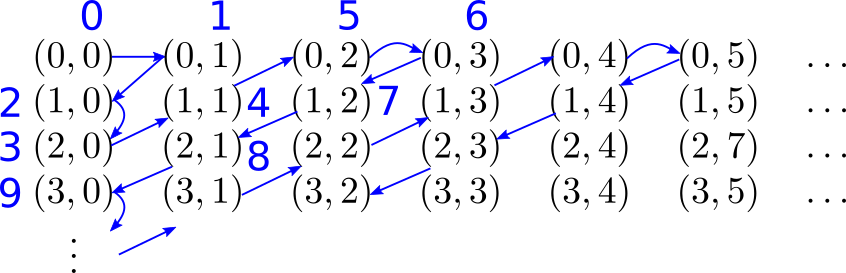
\includegraphics[width=0.70\textwidth]{mapeo_n2yn}
        \caption{Diagonalización de Cantor}
    \end{figure}

    \textit{Noni:} ``Encontrar la fórmula de la función que refleja esto lleva 
    tiempo. Pero la pueden buscar.''

    Hasta acá, obtuvimos que 
    \[ \therefore ~  \#(A\times B)=\#( \mathbb{N} \times \mathbb{N}) =
    \aleph_0 \]

    Pero faltaría probarlo formalmente. 

\end{proof}

\end{enumerate}

\nota{Reescrito con la \fullrefgeneric{subsec:prop-card-lqeq}{%
Propiedad \ref*{subsec:prop-card-lqeq}}}%
\begin{teorema}{Teorema de Bernstein}{bernstein-v2}
Sea $\#A = m$, $\#B = k$.

\[m \leq k \text{ y } k \leq m \implies m = k\]

\end{teorema}

Esto nos dice que teniendo $f: A \to B$ inyectiva y $g: B \to A$ inyectiva,

\begin{gather*}
    \implies \exists \; h: A \to B \text{ biyectiva}
\end{gather*}

La ventaja de este teorema es que trabajamos solamente con funciones 
inyectivas, que son más fáciles de probar que las sobreyectivas.


\begin{proof}
    Usando la \fullrefgeneric{subsec:prop-card-lqeq}{%
    Propiedad \ref*{subsec:prop-card-lqeq}}.
\end{proof}


\subsubsection{Ejemplo}

$\#(\mathbb{N}\times\mathbb{N}) = \aleph_0$
\begin{proof}\phantom{.}
    
    Defino $f: \mathbb{N}\to \mathbb{N} \times \mathbb{N} / f(x) = (x,x)$
    
    $f$ es inyectiva (tarea).
    \begin{gather*}
        \therefore ~ \# \mathbb{N} \leq \# (\mathbb{N} \times \mathbb{N})
    \end{gather*}
    
    Luego, $g: \mathbb{N} \times \mathbb{N} \to \mathbb{N} / g(a,b) = 2^a 3^b$

    \begin{align*}
        g(a,b) = g(c,d) & \\
        \implies& 2^a 3^b = 2^c 3^b \\
        \implies&  a = c \wedge b = d 
        \notamath{Por Teorema Fundamental de la Aritmética (TFA)}
    \end{align*}
    
    Entonces, $g$ es inyectiva y
    $\# (\mathbb{N} \times \mathbb{N}) \leq \mathbb{N}$.
    
    Por el \nameref{teo:bernstein}, 
    $\# \mathbb{N} = \# (\mathbb{N} \times \mathbb{N})$

\end{proof}

\bigskip
\textit{Observación:}
\begin{enumerate}
    \item Cualquier subconjunto de una sección inicial es finito. 

     Es decir, si $A \subseteq I_n \implies A$ es finito.
    \item Si $A \subseteq B$ y $A$ es infinito $\implies B$ es infinito.
\end{enumerate}


\begin{enumerate}
    
    
    \item \begin{proof} Tarea. \nota{\textit{Noni:} ``Recomendación: hacer al 
            finalizar la  teoría de cardinalidad.''}%
    \end{proof}
    \item \begin{proof} \phantom{.}

            Suponiendo que $B$ es finito tenemos dos casos:
            \begin{enumerate}
                \item $B = \varnothing$
                \item $B \sim I_k$ para algún $k \in \mathbb{N}_{\geq 1}$
            \end{enumerate}

            Analicemos cada uno:
            \begin{enumerate}
                \item $A \subseteq B = \varnothing \implies A = \varnothing$
                    $\implies A$ es finito. ¡Absurdo!
                \item $\exists k \in \mathbb{N}_{\geq 1} / 
                    A \subseteq B \sim I_k$

                    \nota{La función inclusión es inyectiva (tarea)}%
                    Por un lado, tenemos la función inclusión: 
                    $inc: A \to B/ inc(a) = a$ 

                    Por otro lado, como
                    $B \sim I_k \implies \exists g: B \to I_k$ biyectiva.

                    \smallskip

                    ¿Qué pasa si componemos $g$ e $inc$?
                    Llamando $h$ a esta función, resulta que
                    $h = g \circ inc: A \to I_k$ es inyectiva por composición
                    de funciones inyectivas.

                    Definamos otra función $\tilde{h}$:

                    \[\tilde{h}: A \to Im(h) \subseteq I_k/\tilde{h}(a)=h(a)\]

                    Notemos que $h$ y $\tilde{h}$ son funciones distintas pues
                    su codominio es diferente.

                    Pero $\tilde{h}$ es biyectiva por ser inyectiva:

                    \begin{gather*}
                        \tilde{h}(a) = \tilde{h}(b) 
                        \implies h(a) = h(b) \implies a = b
                    \end{gather*}

                    Y sobreyectiva:

                    Sea $b \in Im(h)$
                    \begin{align*}
                        &\implies \exists \; a \in A / h(a) = b \\
                        &\implies \tilde{h}(a) = h(a) = b
                    \end{align*}

                    \medskip

                    Por lo tanto, por ser $\tilde{h}$ biyectiva,
                    $\#A = \#Im(h)$
                    y 
                    $Im(h) \subseteq I_k$

                $\underbrace{\implies}_{\substack{\text{Por el item 1}\\%
                \text{ de la observación}}} %
                Im(h)$ es finita
                $\implies$ 
                $A$ es finito. ¡Absurdo!
            \end{enumerate}

            Como el absurdo vino de suponer $B$ finito, entonces $B$ es
            infinito.

        \end{proof}
\end{enumerate}

\bigskip
\textit{Observación:} 
Si $X$ infinito $\implies \exists\; f:\mathbb{N}\to X$ inyectiva.

\medskip

Esta observación nos está diciendo que $\aleph_0 = \# \mathbb{N} \leq \# X$,
es decir, el cardinal más chico de los conjuntos infinitos es $\aleph_0$

\begin{proof}\phantom{.}

    Como $X$ es infinito $\implies X \neq \varnothing \implies \exists \;
    x_0 \in X$.

    Defino $f(0) = x_0$

    \medskip
    Como $X \neq \{x_0\} \sim I_1$ y $X$ es infinito $\implies$ 
    $\exists \; x_1 \in X - \{ x_0 \}$. 

    Defino $f(1) = x_1 \neq x_0$

    Notemos que si
    $X - \{ x_0 \}$ fuera finito 
    $\implies \overbrace{(X-\{x_0\})}^{\text{finito}}
    \cup \overbrace{\{ x_0 \}}^{\text{finito}} = X $ sería finito, lo cual
    es absurdo.
    \nota{Por el ejercicio 3 de la práctica.}%

    \medskip

    Luego $X \neq \{x_0, x_1\} \sim I_2$ y $X$ es infinito $\implies$ 
    $\exists \; x_2 \in X - \{x_0, x_1\}$. 

    Defino $f(2) = x_2$

    Inductivamente,
    $X \neq \{\overbrace{x_0}^{f(0)}, \overbrace{x_1}^{f(1)}, \dotsc, 
    \overbrace{x_n}^{f(n)}\} 
    \sim I_{n+1}$ y $X$ es infinito $\implies$ existe 
    $x_{n+1} \in X - \{f(0), f(1), \dotsc, f(n)\}$. 

    Defino 
    $f(n+1) = x_{n+1} \notin \{ x_0, x_1, \dotsc, x_n \}$


    Y así scesivamente.


    Por último, como cada nueva imagen la elijo en un conjunto donde no están 
    las imágenes anteriores, por definición, $f$ es inyectiva.

\end{proof}


\bigskip
\textit{Observación:}
$A \subseteq B \implies \# A \leq \# B$


\begin{proof} \phantom{.}

    Defino $f: A \to B / f(x) = x$.
    \begin{gather*}
        f(x) = f(y) \implies x = y \\
        \therefore ~ f \text{ es inyectiva}
    \end{gather*}

    Entonces $\# A \leq \# B$.

\end{proof}

\section{Numerable}
\begin{definicion}{Numerable}{}
    \nota{$\# A \leq \mathbb{N}$}%
    $A$ es numerable si $A$ es finito o $A \sim \mathbb{N}$.
\end{definicion}

\subsection{Propiedades}

\begin{enumerate}
    \item $A$ numerable y $A \neq \varnothing 
        \implies \exists \; f:\mathbb{N} \to A$ sobreyectiva.

    \item Si $\exists \; f: \mathbb{N} \to A$ sobreyectiva $\implies A$ es
        numerable.

    \item Si $A$ y $B$ son conjuntos numerables
        $\implies A \times B$ es numerable.
\end{enumerate}

\medskip 

\begin{enumerate}
    \item \begin{proof} Tarea. \end{proof}
    \item \begin{proof} Tarea. \end{proof}
    \item \begin{proof} \phantom{.}

            Como $A$ y $B$ son numerables $\implies$ existen:
            \begin{itemize}
                \item $f_1: \mathbb{N} \to A$ sobreyectiva.
                \item $f_2: \mathbb{N} \to B$ sobreyectiva.
            \end{itemize}

            Luego 
            $f_1 \times f_2 = F: \mathbb{N} \times \mathbb{N} \to A \times B$
            tal que
            \begin{gather*}
                F(n, m) = \left(f_1(n), f_2(m)\right)
            \end{gather*}

            \medskip

            Veamos que $F$ es sobreyectiva.

            Sea $(a,b) \in A \times B$.

            $f_1$ sobreyectiva $\implies$ existe $n \in \mathbb{N}$
            tal que $f_1(n) = a$

            $f_2$ sobreyectiva $\implies$ existe $m \in \mathbb{N}$
            tal que $f_2(m) = b$

            Entonces
            \begin{align*}
                F(n, m) &= \left(f_1(n), f_2(m)\right) = (a,b) \\
                \implies& F \text{ es sobreyectiva} \\
                \implies& \# (
                \underbrace{\mathbb{N} \times \mathbb{N}}_{\aleph_0}
                ) 
                \geq \# (A \times B)
            \end{align*}

            Por lo tanto, $A \times B$ es numerable.
    \end{proof}
\end{enumerate}

\section{Sucesión}

\begin{definicion}{Sucesión}{}
    Una función $f: \mathbb{N} \to A$ es una sucesión de elementos de $A$.

    \bigskip
    \textbf{Notación:} $\left(a_n\right)_{n \in \mathbb{N}}$

    \medskip
    \phantom{\textbf{Notación:}} $\underbrace{f(0)}_{a_0},
    \underbrace{f(1)}_{a_1}, \underbrace{f(2)}_{a_2},
    \underbrace{f(3)}_{a_3}, \dots$
\end{definicion}

\subsubsection{Ejemplo}

\begin{enumerate}
    \item $\begin{cases}
            a_{n+1} = 2 a_n & n \geq 0\\
            a_0 = 1 &
        \end{cases}$

        \[1,2,4,8,16, \dots\]

    \item $a_n = \frac{1}{2^n}$ \nota{$n \in \mathbb{N}$}%

        \[ 1, \frac{1}{2}, \frac{1}{4}, \frac{1}{8} , \dots \]
\end{enumerate}

\section{Proposición}
\begin{proposicion}{}{}
    \[ [0, 1]  = \{ x \in \mathbb{R} / 0 \leq x \leq 1 \} \]

    Es infinito no numerable.
\end{proposicion}

\begin{proof}\phantom{.}

    \begin{enumerate}
        \item $f: \mathbb{N} \to [0,1] / f(x) = \frac{1}{x+1}$ es inyectiva.
            \nota{Tarea}%
            \begin{align*}
                &\implies \# \mathbb{N} \leq \# [0,1] \\
                &\therefore ~ \# [0,1] \geq \aleph_0
            \end{align*}

        \item Supongo que $[0,1]$ es numerable.
            \begin{align*}
                &\implies [0,1] \sim \mathbb{N} \\
                &\implies \exists \; g:\mathbb{N}\to [0,1] \text{ biyectiva}\\
                &\therefore ~ [0,1] = \{ \underbrace{g(0)}_{x_0}, 
                \underbrace{g(1)}_{x_1}, \underbrace{g(2)}_{x_2}, \dotsc \}
            \end{align*}

            \begin{equation*}
                \begin{matrix}
                    x_0 = 0 & x_{00} & x_{01} & x_{02} & x_{03} & x_{04} 
                            & \dots\\
                    x_1 = 0 & x_{10} & x_{11} & x_{12} & x_{13} & x_{14}
                            & \dots \\
                    x_2 = 0 & x_{20} & x_{21} & x_{22} & x_{23} & x_{24}
                            & \dots \\
                \end{matrix}
            \end{equation*}
            
            Con $x_{ij} \in \{0,1,2,3,4,5,6,7,8,9\}$


            Defino $\begin{matrix} 
                d = 0 & d_0 & d_1 & d_2 & d_3 & d_4 & \dots 
            \end{matrix}$,
            \nota{$d_{j} \in \{0,1,2,3,4,5,6,$ $7,8,9\}$}%

            Como $0 \leq d \leq 1 \implies d \in [0,1]$.
            Pero como $d_0 \neq x_{00} \implies d \neq x_0$, 
            $d_1 \neq x_{11} \implies d \neq x_1$, $\dots$,
            $d_n \neq x_{nn} \implies d \neq x_n$

            \begin{gather*}
                \therefore ~ d \notin \{ x_0, x_1, x_2, \dots \}
            \end{gather*}
            \smallskip

            ¡Lo cual es absurdo! Y este vino de suponer que $[0,1]$ es
            numerable.

            \begin{gather*}
                \therefore ~ [0,1] \text{ no es numerable.}
            \end{gather*}
            \smallskip

            Conclusión, el cardinal del $[0,1] > \aleph_0$, pues es un
            conjunto infinito y no numerable.
    \end{enumerate}
\end{proof}

Esta demostración parece ser correcta \textit{pero} contiene un error.

\nota{Repasar sistemas de numeración de Introducción a la Informática.}%
El mismo es que números como $0,23\widehat{9} = 0,24$ son el mismo número 
pero tienen escritura distinta y los estamos comparando como si fueran 
\Verb+string + (cerca del final de la demostración comparamos \Verb+char+ a 
\Verb+char+ los números, $d_0 \neq x_{00} \implies d \neq x_0$)

\medskip
\textit{\textbf{¿Qué números no tienen escritura única?}}

En base 10, los números que tienen colas de ceros se pueden escribir con colas
de nueves.

Por ejemplo, $0,05\widehat{9} = 0,06\widehat{0}$.

\begin{proof}[Parche de la demostración:] \phantom{.}

    Defino $\begin{matrix} 
        d = 0 & d_0 & d_1 & d_2 & d_3 & d_4 & \dots 
    \end{matrix}$ 
    \nota{$d_{j} \in \{1,2,3,4,5,6,$ $7,8\}$}%

    Notar que, como $d$ no tiene ni ceros ni nueves, entonces su escritura es
    única, y puedo compararlos caracter a caracter (decimal a decimal).

\end{proof}

\begin{definicion}{}{}
    \[ \# [0,1] = \mathfrak{C} \]
\end{definicion}

\subsection{Teorema}

\begin{teorema}{}{inf-nonum-cjto-num}
    \begin{enumerate}
        \item Si $X$ es infinito no numerable y $A$ es numerable 
            $\implies X\cup A \sim X$

        \item Si $X$ es infinito no numerable y $A$ es numerable $\implies$
            $X - A \sim X$
    \end{enumerate}
\end{teorema}

\begin{enumerate}
    \item \begin{proof}\phantom{.}

            Como $X$ es infinito $\implies \exists \; f: \mathbb{N} \to X$
            inyectiva.

            \nota{Notemos que $g: \mathbb{N} \to B$ es biyectiva.}%
            Llamamos $B = Im(f) \sim \mathbb{N}$ y $B \subseteq X$

            Luego, 
            \begin{align*}
                Y = X - B & \\
                &\implies X = Y \cup B \\
                &\implies X \cup A = (Y \cup B) \cup A = Y \cup (B \cup A)
            \end{align*}

            \nota{Por el ejercicio 3 de la guía.}%
            $A$ y $B$ numerables $\implies A \cup B$ es numerable.

            Como $B$ es infinito y $B \subset A \cup B \implies A \cup B$
            infinito.

            Como $A\cup B$ es numerable e infinito, entonces 
            $A\cup B \sim \mathbb{N}$ y $B \sim \mathbb{N}$.
    
            \nota{La relación de coordinabilidad es de equivalencia, y, en
                consecuencia, transitiva.}%
            Por lo tanto, por transitividad , resulta que $A \cup B \sim B$
            \[ X \cup A = Y \cup (\underbrace{B \cup A}_{\sim B}) 
            \sim Y \cup B = X \]

            \[ \therefore ~ X \cup A \sim X \]

            \medskip

            Veamos que $Y \cup (B \cup A)  \sim Y \cup B$

            \begin{enumerate}[%
                labelindent=*,
                style=multiline,
                leftmargin=*,
                align=left,
                leftmargin=2\parindent,
                label=Caso \arabic*)]
                \item $A \cap Y = \varnothing$

                    Sea 
                    $H: Y \cup (B \cup A) \to Y \cup B / H(x) = \begin{cases}
                        x & x \in Y \\
                        f(x) & x \notin Y
                    \end{cases}$

                    Como $B \cup A \sim B$, existe $f: B \cup A \to B$
                    biyectiva.

                    \textit{Tarea:} ver que $H$ es biyectiva.

                \item $A \cap Y \neq \varnothing$

                    Podemos reescribir $A$ como 
                    $A = (A \cap Y) \cup (\overbrace{A - Y}^{\widetilde{A}})$,
                    y como $A$ es numerable, cualquier subconjunto lo es. 
                    En particular $\widetilde{A}$ es numerable.


                    Luego, $X \cup \widetilde{A} = X \cup A$. Con esto caigo en
                    el Caso 1, con $\widetilde{A}$ en lugar de $A$.

                    \begin{gather*}
                        \therefore ~ X \cup \widetilde{A} \sim X
                    \end{gather*}

            \end{enumerate}

    \end{proof}


    \item \begin{proof}\phantom{.}

        \begin{enumerate}[%
                labelindent=*,
                style=multiline,
                leftmargin=*,
                align=left,
                leftmargin=2\parindent,
                label=Caso \arabic*)]
            \item $A \subseteq X$

                Tenemos que $X = (X-A) \cup A$, con $A$ numerable.

                \nota{Por ejercicio 3 de la guía.}%
                Si $X-A$ es numerable $\implies (X-A)\cup A$ es numerable
                $\implies X$ es numerable.

                Lo cual es un absurdo. Por lo tanto, $X-A$ no es numerable.
                Entonces, $X-A$ es infinito no numerable.

                \medskip

                Por la proposición anterior, 
                \begin{gather*}
                    (\underbrace{X-A}_{\text{Inf. no num.}}) \cup
                    \underbrace{A}_{\text{Num.}} \sim X-A
                    \implies X \sim X - A
                \end{gather*}


            \item $A \not\subseteq X \implies A = 
                (\underbrace{A \cap X}_{\widetilde{A}}) \cup (A-X)$

                $X-A=X-\widetilde{A}$ y caigo en el Caso 1 con $\widetilde{A}$ en 
                lugar de $A$. \nota{$\widetilde{A} \subseteq X$}%

        \end{enumerate}
    \end{proof}
\end{enumerate}

\subsubsection{Ejemplos}
\begin{itemize}
    \item $\# (0,1) = \mathfrak{C}$

        \begin{proof}\phantom{.}

            \[ \underbrace{[0,1]}_{\text{Inf. no num.}} 
            - \underbrace{\{0,1\}}_{\text{Finito num.}} \sim [0,1] 
        \implies (0,1) 
        \underbrace{\sim}_{\fullref{teo:inf-nonum-cjto-num}}
        [0,1]\]
        \end{proof}

    \item Analogamente, $(0,1] \sim [0,1]$

    \item $\# (-10, 10) = \mathfrak{C}$

        ¡Sí!

        \begin{proof}\phantom{.}
            Veamos que se puede generalizar como $\# (a, b) = \mathfrak{C}$, 
            con $a, b$ números (ninguno es $\infty$).

        \begin{figure}[H]
            \centering
            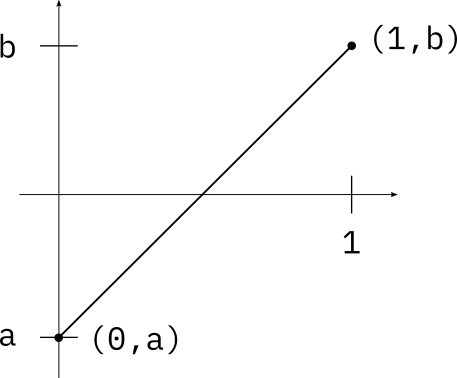
\includegraphics[width=0.45\textwidth]{mapeo_0-1_a-b}
            \caption{$y = (b-a)x + a$}
        \end{figure} \nota{$y=\left(\frac{b-a}{1-0}\right)(x-0)+a$}%

        \[ F: (0,1) \to (a,b) / F(x) = (b-a) x + a \]

        Como $F$ es biyectiva (tarea), entonces $C = \#(0,1) = \#(a,b)$

        \end{proof}

    \item $\# \mathbb{R} = \mathfrak{C}$
        \begin{proof}\phantom{.}
            
            Tomemos la función $\tan{(- \nicefrac{\pi}{2}, \nicefrac{\pi}{2})}
            \to \mathbb{R}$, que es biyectiva.

            Por el item anterior, sabemos que $\# (a,b) = \mathfrak{C}$, 
            entonces:

            \[ \# \left(-\frac{\pi}{2}, \frac{\pi}{2}\right) 
            = \# \mathbb{R} = \mathfrak{C} \]

        \end{proof}
        
        Otra forma de demostrarlo, más analítica es la siguiente:

        \begin{proof}\phantom{.}

            Sea $G: \mathbb{R} \to (-1,1) / G(x) = \frac{x}{1+|x|}$

            Veamos que está bien definida:

            \[ |G(x)| = \left| \frac{x}{1+|x|} \right| 
            = \frac{|x|}{1+|x|} < 1 \iff |x| < 1 + |x| \]

            Para probar que $G$ es biyectiva (tarea), podemos tomar dos 
            caminos:

            \begin{enumerate}
                \item Probar que $G$ es inyectiva y sobreyectiva.
                \item Probar $H: (-1,1) \to \mathbb{R} / 
                    H(x) = \frac{x}{1-|x|}$ es la inversa de $G$
            \end{enumerate}
            
        \end{proof}
\end{itemize}


\section{Teorema de Cantor}

\begin{teorema}{Teorema de Cantor}{cantor}
    Dado $X$ un conjunto, $\# X < \# \mathcal{P}(X)$
\end{teorema}


Este teorema nos está diciendo que:
\[ \# \mathbb{N} = \aleph_0
    < \# \mathcal{P}(\mathbb{N})
    < \# \mathcal{P}(\mathcal{P}(\mathbb{N}))
    < \# \mathcal{P}(\mathcal{P}(\mathcal{P}(\mathbb{N})))
    < \dots \]

Es decir, hay infinitos cardinales distintos correspondientes a conjuntos
infinitos.

\begin{proof} \phantom{.}

    Sea $F: X \to \mathcal{P}(X) / F(a) = \{a\} \subseteq X$
    \begin{gather*}
        F(a) = F(b) \implies \{a\} = \{b\} \implies a = b \\
        \therefore ~ F\text{ es inyectiva.}
    \end{gather*}

    Por esto, $\# X \leq \# \mathcal{P}(X)$

    \nota{Recordar:
    $\#A \geq \#B$
    $\iff$
    $\exists \; f: A \to B$ sobreyectiva}%
    Para ver que es menor estricto, tenemos que ver que no existe ninguna 
    función sobreyectiva de $X$ en $\mathcal{P}(X)$, ya que esto implica
    que no puede ser mayor o igual.

    Supongo que existe $g: X \to \mathcal{P}(X)$ sobreyectiva.

    $B = \{ a \in X / a \notin g(a) \} \subseteq X
    \quad \therefore ~ B \in \mathcal{P}(X)$ 

    \medskip
    Notemos que $g(x)$ ($g$ evaluada en $x$) es un conjunto.

    Por ejemplo, si tuviéramos una función
    $g: \mathbb{N} \to \mathcal{P}(\mathbb{N})$ tal que:
    \begin{gather*}
    g(3) = \{1,2,4\}, \quad g(5) = \{5,6\} \\
    \\
    3 \notin g(3), \; 5 \in g(5) \\ \implies 3 \in B, 5 \notin B
    \end{gather*}

    \medskip

    Como la función $g$ es sobreyectiva $\implies$ existe $b \in X$ tal que
    $g(b) = B$

    Naturalmente surge la pregunta de quiénes son los $b \in B$.
    \[ b \in B \underbrace{\iff }_{\text{Def. } B} b \notin g(b) 
        \underbrace{\iff}_{g(b)=B} b \notin B \]

    ¡Absurdo! Vino de suponer que existe una $g$ sobreyectiva.
    \begin{align*} 
        \therefore ~ &\nexists \; g:X \to\mathcal{P}(X) \text{ sobreyectiva}\\
        &\implies \# X \not\geq \# \mathcal{P}(X) \\
        &\implies \# X < \# \mathcal{P}(X)
    \end{align*}
\end{proof}

\section{Álgebra de cardinales}

\begin{definicion}{Álgebra de Cardinales}{}
    Sean $a = Card(X)$ y $b = Card(Y)$

    Definimos
    \begin{enumerate}
        \item $a + b = \# (X \cup Y)$, con $X \cap Y = \varnothing$
        \item $a \cdot b = \# (X \times Y)$
        \item $a^b = \# \{ f: Y \to X / f $ es función
            $\} = \# \left({X}^{Y}\right)$
            \nota{$X \neq \varnothing$, $Y \neq \varnothing$}%
    \end{enumerate}

\end{definicion}

\begin{proof} Buena definición.

    \begin{enumerate}
        \item Sea $\underbrace{\widetilde{X} \sim X}_{\# \widetilde{X} = a}$.

            Sea $\underbrace{\widetilde{Y} \sim Y}_{\# \widetilde{Y} = b}$ 
            tal que
            $\widetilde{X} \cap \widetilde{Y} = \varnothing$

            Quiero ver que 
            $\# (\widetilde{X} \cup \widetilde{Y}) = \# (X \cup Y)$

            \begin{align*}
                \widetilde{X} \sim X & \implies \exists \;
                f: \widetilde{X} \to X
                \text{ biyectiva}\\
                \widetilde{Y} \sim Y & \implies \exists \;
                g: \widetilde{Y} \to Y
                \text{ biyectiva}\\
            \end{align*}

            Defino $H: \widetilde{X} \cup \widetilde{Y} \to X \cup Y/$ 
            \nota{Buena definición pues 
            $\widetilde{X}\cap\widetilde{Y}=\varnothing$}%
            $H(z) = \begin{cases}
                f(z) & \text{si } z \in \widetilde{X} \\
                g(z) & \text{si } z \in \widetilde{Y} \\
            \end{cases}$

            Tarea: $H$ es biyectiva.

        \item Defino $m \, . \, n = \# (X \times Y)$

            Tarea: probar la buena definición.

        \item Defino $X \neq \varnothing$, $Y \neq \varnothing$.

            \begin{gather*}
                m^{n} = \# \{ f: Y \to X / f \text{ es función} \} = \# X^{Y}
            \end{gather*}

            Veamos que está bien definida.

            
            % Puesta acá para correcta alineación con la página
            \nota{Notemos que los elementos de ${X}^{Y}$ son funciones de $Y$
                en $X$; y los de ${\widetilde{X}}^{\widetilde{Y}}$ son 
                funciones de $\widetilde{Y}$ en $\widetilde{X}$.}%
            \begin{align*}
                \widetilde{X}\sim X &\implies \exists \; f: \widetilde{X} 
                \to X \text{ biyectiva}  \\
                \widetilde{Y}\sim Y &\implies \exists \; g: \widetilde{Y} 
                \to Y  \text{ biyectiva}
            \end{align*}

            Veamos que ${X}^{Y} \sim {\widetilde{X}}^{\widetilde{Y}}$

           \medskip

             Defino $H: {X}^{Y} \to {\widetilde{X}}^{\widetilde{Y}} / H(F)=G$,
            siendo
            $G(a) = f^{-1} \circ F \circ g(a) \in \widetilde{X}$, con 
            $a \in \widetilde{Y}$

            \begin{itemize}
                \item Inyectividad)
                    \begin{align*}
                        H(F_1) = H(F_2) & \\
                        &\implies G_1 = G_2 \\
                        &\implies G_1(a) = G_2(a)
                        \notamath{$\forall a \in \widetilde{Y}$} \\
                        &\implies f^{-1}\circ F_1 \circ g(a) =
                        f^{-1} \circ F_2 \circ g(a) 
                        \notamath{$\forall a \in \widetilde{Y}$} \\
                        &\implies \underbrace{f \circ f^{-1}}_{id} 
                        \circ F_1 \circ g(a) =
                        \underbrace{f \circ f^{-1}}_{id} 
                        \circ F_2 \circ g(a)
                        \notamath{$f$ es biyectiva. 
                            $\forall a \in \widetilde{Y}$} \\
                        &\implies F_1(g(a)) = F_2(g(a))
                        \notamath{$\forall a \in \widetilde{Y}$}
                    \end{align*}

                    Luego, $F_1, F_2 : Y \to X$

                    Queremos ver que $F_1(y) = F_2(y)$, $\forall y \in Y$

                    Sea $y \in Y \implies \exists z \in \widetilde{Y}/g(z)=y$,
                    pues $g$ es sobreyectiva.

                    Como $F_1(g(a)) = F_2(g(a))$, entonces
                    $F_1(\underbrace{g(z)}_{y}) = F_2(\underbrace{g(z)}_{y})$

                    \begin{gather*}
                        \therefore ~ F_1 = F_2
                    \end{gather*}

                    En conclusión, $H$ es inyectiva.

                \item Sobreyectividad) Tarea.
            \end{itemize}

    \end{enumerate}

\end{proof}

\subsubsection{Ejemplos}
\begin{itemize}
\item \begin{align*}
    2 + 3 &= 
    \# \left(\{\circ, \bigtriangleup\} \cup \{x_1,x_2,x_3\}\right) \\
    & = \# \left(\{\circ, \bigtriangleup, x_1,x_2,x_3\}\right) \\
    &= 5
\end{align*}

\textit{``¡Oh! ¡Qué novedad! ¡$2+3=5$!''} 

Sí, es novedoso porque acá estamos hablando de \textit{cardinales}.
Sus símbolos coinciden con los de los números, pero no significan lo
mismo.

La ventaja es que si los símbolos coinciden con los de los números,
su suma también lo hace.

\item $\# \{ \mathbb{N} \to \{-1,1\} / f \text{ es función} \} 
    = {(\#\{-1,1\})}^{\mathbb{N}} = 2^{\aleph_0}$

    \item $\# (\mathbb{N}\times\mathbb{N}) =  \mathbb{N} \cdot \mathbb{N} 
        = \aleph_0 \cdot \aleph_0$ y, como 
        $\# (\mathbb{N} \times \mathbb{N}) = \# \mathbb{N} = \aleph_0 $, entonces 
        $\aleph_0 \cdot \aleph_0 = \aleph_0$
\end{itemize}

\subsection{Propiedad}
\begin{gather*}
    \# \mathcal{P}(X) = 2^{\# X}
\end{gather*}

% Puesta acá para correcta alineación con la página
\nota{\textit{Noni:} ``En matemática parece un poco extraño, pero en
programación lo hacemos naturalmente: definimos funciones que reciben
cualquier argumento y devuelven otra función.''}%
\begin{proof}\phantom{.}

    Sea $Y = \{f: X \to \{0,1\} / f \text{ es función} \}$, por las
    definiciones vistas anteriormente $\# Y = 2^{\# X}$

    $F: \underbrace{\mathcal{P}(X)}_{\text{Conjuntos}} 
    \to \underbrace{Y}_{\text{Funciones}} / 
    F(\text{conjunto}) = \text{función}$

    \medskip

    Definamos $F(A) = \Chi_A$

    \begin{itemize}
        \item Iny.) 
            % Puesta acá para correcta alineación con la página
            \nota{$\Chi_A$ es la función característica de A.\\
                Recordemos que se define como: \\
            $\Chi_A: X \to \{0,1\}/$ $\Chi_A (t) = \begin{cases}
                1 & t \in A \\ 0 & t \notin A
            \end{cases}$}%
            $F(A) = F(B) \implies \Chi_A = \Chi_B 
            \implies \Chi_A (t) \underbrace{=}_{*} 
            \Chi_B (t) $, $\forall t \in X$
           \begin{align*}
               \text{Sea } t \in A \phantom{\iff} & \\
               \iff &\Chi_A (t) = 1 \\
               \underbrace{\iff}_{*} &\Chi_B (t) = 1 \\
               \iff & t \in B
           \end{align*}
           \begin{gather*}
               \therefore ~  t \in A \iff t \in B
           \end{gather*}

           Entonces $A = B$.
       \item Sobrey.) Sea $h \in Y$.

           Defino $C = \{ x \in X / h(x) = 1 \} \subseteq Y$

           Entonces $C \in \mathcal{P}(x)$ y tiene sentido hacer 
           $F(C) \implies F(C) = \Chi_C$

           \bigskip
           Veamos que $\Chi_C = h$

           Sea $t \in X_C$.
           \begin{align*}
               \Chi_C (t) = 1 & \\
               & \iff t \in C \\
               & \iff h(t) = 1 \notamath{Definición de $C$} \\
            \end{align*}

            Es decir, \dashbox{$\Chi_C (t) = 1 \iff h(t) = 1$}

            Lo cual es equivalente a decir que 
            $\Chi_C (t) \neq 1 \iff h(t)\neq 1$, que a su vez es equivalente a
            $\Chi_C (t) = 0 \iff h(t) = 0$

            \[ \therefore ~ \Chi_C = h \]
    \end{itemize}
    Conclusión, $F$ es biyectiva 
    $\implies \# \mathcal{P}(x) = \# Y = 2^{\# X}$

\end{proof}


\subsection{Teorema}

\begin{teorema}{}{}
    \begin{gather*}
        2^{\aleph_0} = \mathfrak{C}
    \end{gather*}
\end{teorema}

\begin{proof}\phantom{.}

    Sea
    $U = [0,1] \implies \# U = \mathfrak{C}$

    Sea
    $T = {\{0,1\}}^{\mathbb{N}}
    = \{f:\mathbb{N} \to \{0,1\}/f \text{ es función}\}
    \implies \# T=2^{\aleph_0}$


    \nota{Interpreto el número en base 2.}%
    Defino $F: T \to U / F(a_0 a_1 a_2 a_3 \dots) = {(0,a_0 a_1 a_2 a_3 )}_2$

    \begin{gather*}
        a_0 a_1 a_2 a_3 \dots \mapsto \notamath{$(0,1)_2 
                                    = \nicefrac{1}{2} = 0,5$}%
        x = \sum_{k=1}^{\infty} \frac{a_{k-1}}{2^k}
    \end{gather*}

    \begin{align*}
        F(a_0 a_1 a_2 \dots) &= F(b_0 b_1 b_2 \dots)  \\
        &\implies (0, a_0 a_1 a_2 \dots)_2 = (0, b_0 b_1 b_2 \dots)_2 \\
        & \underbrace{\implies}_{\text{Mal}} 
        a_j = b_j \; \forall j \in \mathbb{N} \notamath{Esta 
            implicación está mal porque en base 2 los números no tienen
            escritura única.\\$0,010\widehat{1}=0,011$} \\
        &\implies a_0 a_1 a_2  \dots = b_0 b_1 b_2  \dots
    \end{align*}

    Así como está escrita, $F$ no es inyectiva pues 
    \[F(01011111 \dots) = F(01100000 \dots)\]

    \phantom{.}

    Para arreglar esto, definimos 
    $T_0 = \{ f \in T / f \text{ tiene colas de ceros}\}$, o lo que es lo
    mismo, $T_0 = \{ f \in T / 
    f(x) = 0 ~ \forall k \vee f(k) = 0 ~ \forall k \geq j \text{ y } f(j-1)=1 \}$

    Definimos también
    $G: T_0 \to \mathbb{N} / G(a_0 a_1 \dots a_{j-1} 0 \dots 0) 
    = 1 a_0 a_1 \dots a_{j-1}$

    $G$ es inyectiva:
    \begin{align*}
        G(a_0 a_1 \dots a_{j-1} 0 \dots 0) &= 
        G(b_0 b_1 \dots b_{t-1} 0 \dots 0) \\
        &= 1 a_0 a_1 \dots a_{j-1} = 1 b_0 b_1 \dots b_{t-1} \\
        &\implies a_i = b_i \forall \, i \\
        &\implies G \text{ es inyectiva} \\
        &\implies \# T_0 < \# \mathbb{N} = \aleph_0 \\
        &\implies T_0 \text{ es numerable} \\
        \\
        & \therefore ~ \# (T-T_0) = \# T = 2^{\aleph_0}
        \notamath{ $T-T_0\sim T$\\ Con $T$
            infinito no numerable, pues $2^{\aleph_0} > \aleph_0$ 
        (por el \nameref{teo:cantor}), $T_0$ numerable y, en consecuencia,
        $\# T = 2^{\aleph_0}$. }
    \end{align*}

    \phantom{.}

    Defino ahora $F: (T-T_0) \to U / F(a_0 a_1 \dots a_{j-1} 0 \dots 0)
    = (0, a_0 a_1 \dots )_2 $

    Estos números sí tienen escritura única pues no hay colas de ceros.
    Solucionamos así el problema de la inyectividad.

    \begin{align*}
        F(a_0 a_1 a_2 \dots) &= F(b_0 b_1 b_2 \dots) \\
        &\implies (0, a_0 a_1 a_2 \dots)_2 = (0, b_0 b_1 b_2 \dots)_2 \\
        & \implies
        a_j = b_j \; \forall j \in \mathbb{N} \notamath{Al no tener cola
        de ceros, tienen escritura única} \\
        & \therefore ~ F \text{ es inyectiva}
    \end{align*}

    \[ \dashbox{$\# (T-T_0) \leq \# U$} \]

    Ahora la sobreyectividad.

    Para ella, notamos un problema: al sacar las colas de ceros, también 
    sacamos al cero. En consecuencia, el cero no va a estar en la imagen y
    la función no va a ser sobreyectiva.

    \begin{gather*}
        \widetilde{U} = (0,1] \sim [0,1] - \{ 0 \} \\
        \therefore ~ \# \widetilde{U} = \mathfrak{C}
    \end{gather*}

    Queda entonces definida \nota{Con $\widetilde{U} = (0,1]$}%

    $F: (T-T_0) \to \widetilde{U} / F(a_0 a_1 \dots a_{j-1} 0 \dots 0)
    = (0, a_0 a_1 \dots )_2 $


    Con esto, $F$ es sobreyectiva:

    
    \begin{gather*}
        x \in \widetilde{U} \implies x = (
        \underbrace{0, u_0 u_1 u_2 u_3 u_4 u_5 \dots}_{\substack{
            \text{Lo escribo de forma tal} \\
            \text{que no tenga cola de ceros.}
        }})_2 \notamath{$(0,1)_2 = (0,0\widehat{1})_2$}%
        \\ \\
        \therefore ~ F(u_0 u_1 u_2 \dots) = x
    \end{gather*}

    Conclusión, $F$ es biyectiva y, en consecuencia,
    $\# (T-T_0) = \# \widetilde{U}$.

    Como $\#(T-T_0) = 2^{\aleph_0}$ y $\# \widetilde{U} = \mathfrak{C}$, 
    queda probado que

    \[ \boxed{2^{\aleph_0} = \mathfrak{C}} \]

\end{proof}

\subsubsection{Ejemplo}

Calcular ${\aleph_0}^{\aleph_0}$

\begin{align*}
    2 \leq \aleph_0 \leq C & \\
    &\implies \notamath{Por ej. de la guía}
    2^{\aleph_0} \leq {\aleph_0}^{\aleph_0} 
    \leq {C}^{\aleph_0} = {\left(2^{\aleph_0}\right)}^{\aleph_0} \\
    &\implies \notamath{Por ej. de la guía: 
    $\left(2^x\right)^y = 2^{xy}$}
    2^{\aleph_0} \leq {\aleph_0}^{\aleph_0} \leq 2^{\aleph_0 \cdot \aleph_0}
    = 2^{\aleph_0} \\
    &\implies C \leq {\aleph_0}^{\aleph_0} \leq C \\
    &\implies \boxed{{\aleph_0}^{\aleph_0} = \mathfrak{C}}
\end{align*}

\section{Hipótesis del continuo}

\nota{\textit{Noni:} ``Es una \textit{hipótesis} y no un \textit{teorema} pues
no hay demostración de que este conjunto exista o no, pero la comunidad
matemática acuerda construir sobre esto.''}%
\begin{hipotesis}{Hipótesis del continuo}{}
    \[ \nexists \; X \text{ conjunto tal que } \aleph_0 < \# X < C \]
\end{hipotesis}

La hipótesis está diciendo que no hay ningún conjunto entre $\aleph_0$ y $C$.

\section{Truco visto en la práctica}

\begin{itemize}
    \item En algunos problemas podemos definir 
        \begin{gather*}
            f : A \to B / f(x) = x
        \end{gather*}
        Y demostrar fácilmente que $f$ es inyectiva.
\end{itemize}
